\chapter{Introduction}\label{chapter:introduction}
The software architecture is the set of principles assisting software architects and developers for system or application design \cite{Dashofy:2009aa}. It defines a process to decompose a system into modules, components and specifies their interactions \cite{Brown:2015aa}. In this chapter, two different architectural approaches, namely monolithic architectural approach and microservices achitectural approach, are discussed. Firstly, a conceptual understanding of the monolithic architecture approach is presented, which is followed by its various advantages and disadvantages. Secondly, an overview of the microservices architecture approach is explained. In Section \ref{section:context/motivation}, the motivation for the current research is discussed which is then followed by a list of research questions. Finally, in Section \ref{section:context/approach} and Section \ref{section:context/research_strategy}, the approach that is used to conduct the current research is presented. The purpose of this chapter is to provide a basic background context for the following chapters.

\section{Monolithic Architectural Approach}\label{section:context/monolith}
A mononlithic architectural approach is one in which even a modular application is deployed as a single artifact. Figure \ref{fig:context/monolith-example} shows the architecture of an Online-Store application that has a clear separation of components such as Catalog, Order etc., as well as respective models such as Product, Order etc. Despite the modular decomposition of the application, all the components are deployed as a single application artifact on the server.\cite{Richardson:2014aa}\cite{Richardson:2014ab}

\begin{figure}[H]
\begin{center}
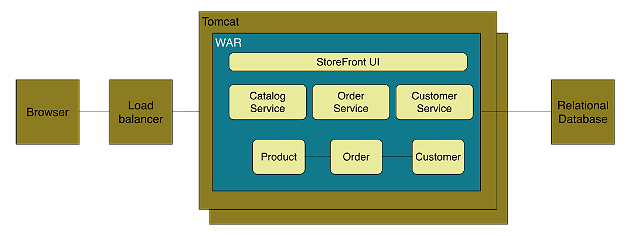
\includegraphics[width=0.7\textwidth]{figures/context-monolith-example}
\caption{Monolith Example from \cite{Richardson:2014aa}}
\label{fig:context/monolith-example}
\end{center}
\end{figure}


\subsection{Types of the Monolithic Architectural Approach}\label{subsection:context/monolith-types}
According to \cite{Annett:2014aa}, a monolith can be of several types depending upon the viewpoint, as shown below:
\begin{enumerate}
\item \textbf{Module Monolith}: If all the code to realize an application share the same codebase and need to be compiled together to create a single artifact for the whole application then the architecture is called Module Monolithic Architecture. An example of this architecture is shown in Figure \ref{fig:context/module-monolith-example}. The application on the left side of the figure, has all the code in the same codebase in the form of packages and classes without clear definition of modules and gets compiled to a single artifact. However, the application on the right side is developed as a number of modular codebase, each has separate codebase and can be compiled to different artifact. In the application shown in the left side of the figure, the various parts of the codebase can reference each other directly.

\begin{figure}[H]
\begin{center}
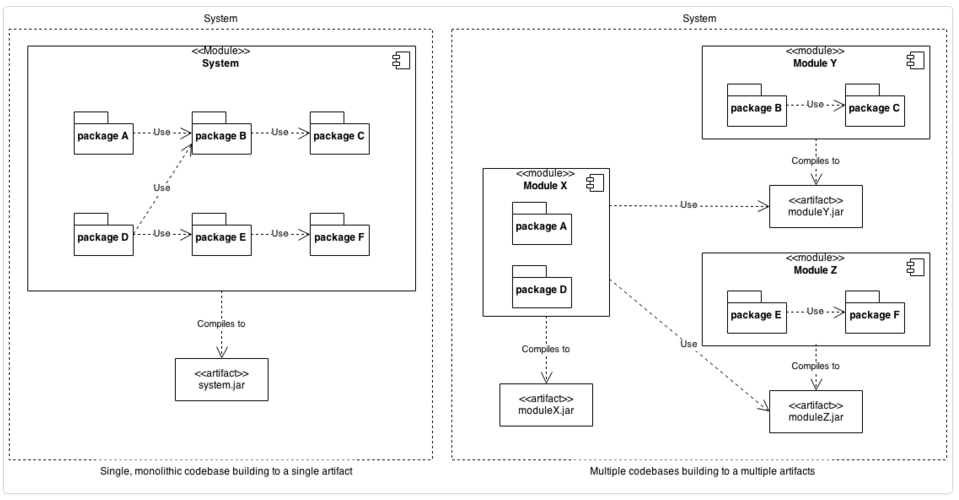
\includegraphics[width=0.8\textwidth]{figures/context-module-monolith}
\caption{Module Monolith-Example from \cite{Annett:2014aa}}
\label{fig:context/module-monolith-example}
\end{center}
\end{figure}

\\
\item \textbf{Allocation Monolith}: An Allocation Monolith is created when code is deployed to all the servers as a single version. This means that all the components running on the servers have the same version at any time. The Figure \ref{fig:context/allocation-monolith-example} gives an example of the allocation monolith. The system on the left side of Figure \ref{fig:context/allocation-monolith-example} has the same version of the artifact for all the components on all the servers. It does not make any difference whether or not the system has a single codebase and artifact. However, the system on the right as shown in the figure is realized with multiple versions of the artifacts in different servers at any time.

\begin{figure}[H]
\begin{center}
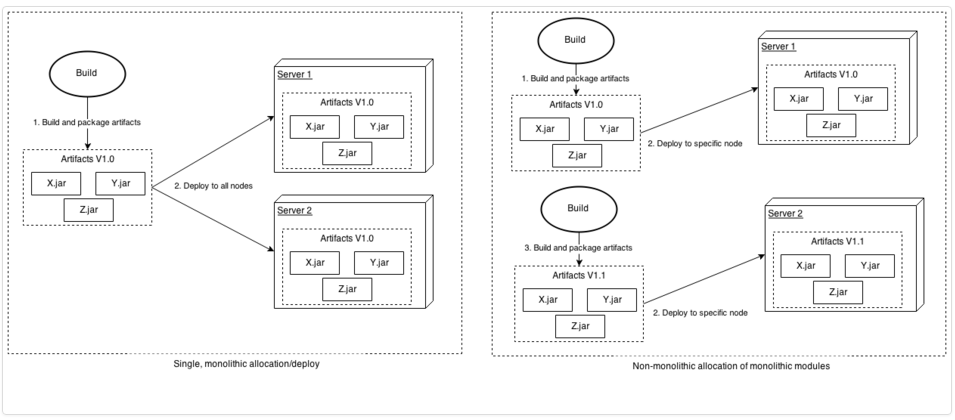
\includegraphics[width=0.8\textwidth]{figures/context-allocation-monolith}
\caption{Allocation Monolith-Example from \cite{Annett:2014aa}}
\label{fig:context/allocation-monolith-example}
\end{center}
\end{figure}

\\
\item \textbf{Runtime Monolith}: In the runtime monolith, the whole application is run under a single process. The application on the left side of Figure \ref{fig:context/runtime-monolith-example} shows an example of runtime monolith where a single server process is responsible for the whole application. Whereas the application on the right has allocated multiple server processes to run distinct set of component artifacts of the application.

\begin{figure}[H]
\begin{center}
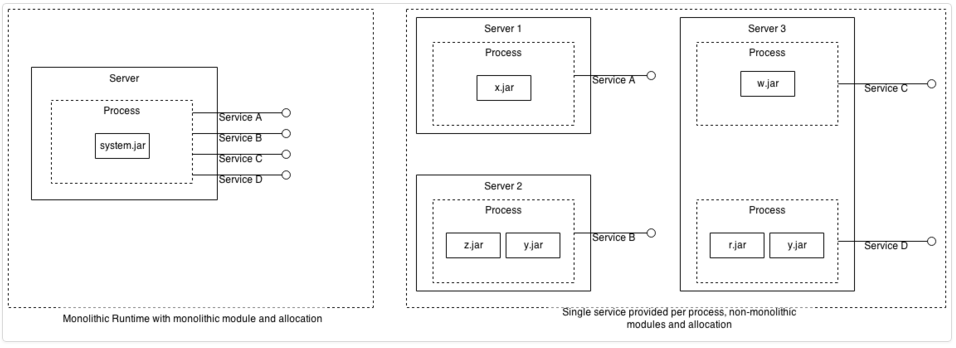
\includegraphics[width=0.8\textwidth]{figures/context-runtime-monolith}
\caption{Runtime Monolith-Example from \cite{Annett:2014aa}}
\label{fig:context/runtime-monolith-example}
\end{center}
\end{figure}
\end{enumerate}

\\
\subsection{Advantages of the Monolithic Architectural Approach}\label{subsection:context/monolith-advantages}
The monolithic architectural approach is appropriate for small applications and has the following benefits \cite{Richardson:2014ab}\cite{Fowler:2014aa}\cite{Gupta:2015aa}\cite{Abram:2014aa} :
\begin{itemize}[leftmargin=.5in]
\item It is easy to develop a monolith application since various development tools including \acrshort{IDE}s are created around the single application concept. Furthermore, it is also easy to test the application by creating appropriate environment on the developer's machine.
\item The deployment can be simply achieved by moving the single artifact for the application to an appropriate directory in the server.
\item The scaling can be clearly and easily done by replicating the application horizontally across multiple servers behind a load balancer as shown in Figure \ref{fig:context/monolith-example}
\item The different teams are working on the same codebase so sharing the functionality can be easier.
\end{itemize}
\\
\subsection{Disadvantages of the Monolithic Architectural Approach}\label{subsection:context/monolith-disadvantages}
As the requirements of the system grows over time, the corresponding system's codebase becomes large and the size of team increases. Under such circumstances, the monolithic architecture faces many challenges as explained below:
\\
\cite{Namiot:2014aa}\cite{Newman:2015aa}\cite{Abram:2014aa}\cite{Richardson:2014aa}\cite{Richardson:2014ab}\cite{Gupta:2015aa}
\begin{itemize}[leftmargin=.5in]
\item \textbf{Limited Agility}: As the whole application has a single codebase, even changing a small feature to release it in the production takes time. Firstly, a small change can trigger changes to other dependent code. In huge monolithic applications, it is very difficult to manage modularity especially when all the team members are working on the same codebase. Secondly, to deploy a small change in the production, the whole application has to be deployed. Thus continuous delivery gets slower. This is more problematic when multiple changes have to be released on a daily basis. The slow pace and low frequency of release will highly affect agility.
\\
\item \textbf{Decrease in Productivity}: It is difficult to understand the application especially for a new developer because of the size of codebase. Although it also depends upon the structure of the codebase, it will still be difficult to grasp the significance of the code when there is no hard modular boundary. Additionally, a developer can be intimidated due to need to see the whole application at once from outwards to inwards direction. Secondly, the development environment can be slow to load the whole application and at the same time the deployment will also be slow. Overall, it will slow down the speed of understandability, execution and testing.
\\
\item \textbf{Difficult Team Structure}: The division of a team as well as assigning tasks to the team members can be challenging. Most common ways to partition teams in monolithic architectureal approach are by technology and by geography. However, partitioning either by technology or by geography may not be appropriate in all cases. In any case, the communication among the teams can be difficult and slow. Additionally, it is not easy to assign complete vertical ownership to a team for a particular feature from development to release. If something goes wrong in the deployment, there is always a question who should find the problem, is it either the operations team or the last person who commited the code. The approprate team structure and the ownership of code are very important for agility.
\\
\item \textbf{Long Term Commitment to Technology stack}: The technology to use is chosen before the development phase by analysing the requirements and the maturity of current technology at that time. All the teams in the project need to follow the same techonology stack throughout the lifecycle of an application. However, if the requirement changes then there can be situations when specific features can be best solved by different set of technologies. Additionally, not all the features in the application are the same and hence cannot be solved using same technology. Nevertheless, the technology advances rapidly. So, the solution thought right at the time of planning can be outdated and there can be a better solution available at present. In monolithic applications, it is very difficult to migrate to a newer technology stack and it can rather be a painfull process.
\\
\item \textbf{Limited Scalability}: The scaling of monolith application can be performed in either of two ways. The first way is to replicate the application along many servers and dividing the incoming request using a load balancer in front of the servers. Another approach is using identical copies of the application in multiple servers as in previous case but partitioning the database access instead of user request. Both of these scaling approaches improves the capacity and availability of the application. However, the individual requirement regarding scaling for each component can be different but cannot be fulfilled with this approach. Also, the complexity of the monolith application remains the same because we are replicating the whole application. Additionally, if there is a problem in a component the same problem can affect all the servers running the copies of the application, this does not improve resilency.\cite{MacVittie:2014aa}\cite{Namiot:2014aa}
\end{itemize}
\\

\section{Microservices Architectural Approach}\label{section:context/microservices_architecture_style}
With monolith, it is easy to start development. But as the system gets bigger and complicated over time, it becomes very difficult to be agile and productive. The disadvantages listed in Section \ref{subsection:context/monolith-disadvantages} outweighs its advantages as the system gets old. The various qualities such as scalability and agility need to be maintained for the whole lifetime of the application. It becomes complicated due to the fact that the system needs to be updated continuously as the as the requirements keep changing and evolving over time. In order to tackle these disadvantages, microservices architecture style is followed.\\
The microservices architecture uses the approach of decomposing an application into smaller autonomous components. The following Section \ref{section:context/microservices_architecture_style/decompostion_of_an_application} provides details of the various decomposition techniques.

\subsection{Decomposition of an Application}\label{section:context/microservices_architecture_style/decompostion_of_an_application}
There are various ways to decompose an application. This section discuss two different ways of breaking down an application.

\subsubsection{Scale Cube}\label{section:context/microservices_architecture_style/decompostion_of_an_application/scale_cube}
The Section \ref{subsection:context/monolith-disadvantages} captured various disadvantages related to the monolithic architectural approach. In \cite{Fisher:2015aa}, authors propose an approach called scale cube to address the challenges related to agility, scalability and productivity. The scale cube provides three dimensions of scalability as shown in Figure \ref{fig:context/scale-cube} which can be applied alone or simultaneously depending upon the situation and desired goals of the system.

\begin{figure}[H]
\begin{center}
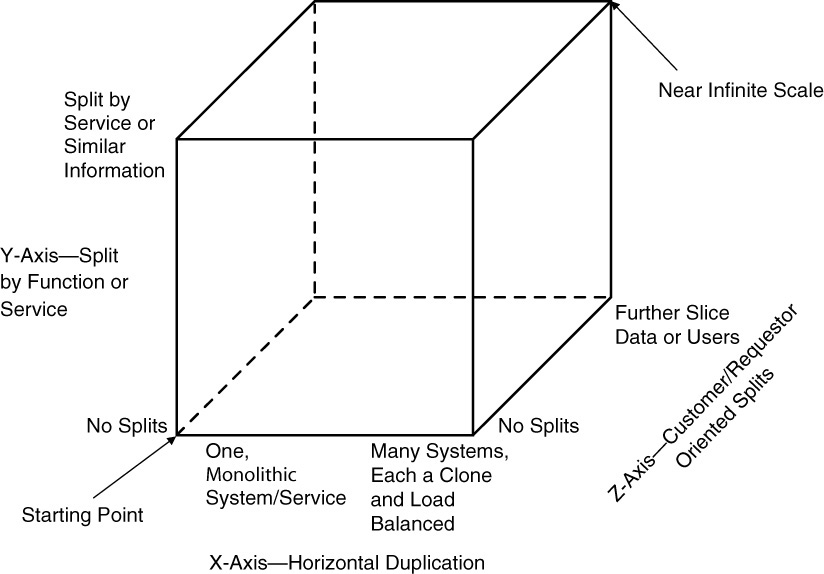
\includegraphics[width=0.5\textwidth]{figures/context-scale-cube}
\caption{Scale Cube from \cite{Fisher:2015aa}}}
\label{fig:context/scale-cube}
\end{center}
\end{figure}

\\
The scaling along each dimensions are described below. \cite{Fisher:2015aa}\cite{MacVittie:2014aa}\cite{Richardson:2014aa}
\begin{enumerate}
\item X-axis Scaling: It is achieved by cloning the application and data along multiple servers. A pool of requests are sent to a load balancer and the requests are deligated to the servers. Each of the servers has the latest version of the application and access to all the data required. In this respect, it does not make any difference which server fulfills the request. Rather, it is about how many requests are fulfilled at any time. It is easy to scale along X-axis as the number of requests increases. The solution is as simple as to add additional clones. However, with this type of scaling, it does not scale with the increase in data. Moreover, it also does not scale when there are large variation in the frequency of any type of requests because all the requests are handled in an unbiased way and allocated to servers in the same way.
\\
\item Z-axis Scaling: The scaling is obtained by spliting the request based on certain criteria or information regarding the requestor or customer affected by the request. It is different than X-axis scaling in the way that the servers are responsible for different kinds of requests. Normally, the servers have the same copy of the application but some can have additional functionalies depending upon the requests expected. The Z-axis scaling helps in fault isolation and transaction scalability. Using this scaling, certain group of customers can be provided additional functionalities. Additionally, a new functionality can be tested to a small group of customers to minimize the risk.
\\
\item Y-axis Scaling: The scaling along this dimension means the spliting of the application's responsibility. The separation can be done either by data, by the actions performed on the data or by the combination of both. The respective ways can be referred to as resoure-oriented or service-oriented splits. While the x-axis or z-axis split are rather duplication of work along servers, y-axis is more about specialization of work along servers. The major advantage of this scaling is that each request is scaled and handled differently according to its necessity. As the logic along with the data to be worked on are separated, developers can focus and work on small section at a time. This will increase productivity as well as agility. Additionally, a fault in a component is isolated and can be handled gracefully without affecting rest of the application. However, scaling along Y-axis can be costly compared to scaling along other dimensions.
\end{enumerate}
\subsubsection{Shared Libraries}\label{section:context/microservices_architecture_style/decompostion_of_an_application/shared_libraries}
Libraries are a standard way of sharing functionalities among various services and teams. This capability is provided as a feature of the programming languages. The shared libraries however do not provide technology heterogeneity. Furthermore,  a) independent scaling b) independent deployment and c) independent maintainance cannot be achieved unless the libraries are dynamically linked. In such cases, any small change in the library leads to redeployment of the whole system. Moreover, sharing the code is a form of coupling and should be avoided.

Decomposing an application into individual features gives various advantages such that each feature can be a) scaled independently b) deployed independently c) agile and d) assigned easily to teams. Microservices use the decomposition technique proposed by the scale cube. The detail advantages of microservices architectural approach are discussed further in Section \ref{section:challanges_of_microservices_architecture/introduction/challenges}.
\subsection{Definitions}\label{section:context/microservices_architecture_style/definitions}
There are several definitions given by several pioneers and early adapters of the microservices architectural approach.
\\
\begin{shaded}Definition 1: \cite{Richardson:2014ac} \end{shaded}
"It is the way to functionally decompose an application into a set of collaborating services, each with a set of narrow, related functions, developed and deployed independently, with its own database."

\\
\begin{shaded}Definition 2: \cite{Wootton:2014aa}\end{shaded}
"It is a style of software architecture that involves delivering systems as a set of very small, granular, independent collaborating services."


\\
\begin{shaded}Definition 3: \cite{Cockcroft:2015aa}\end{shaded}
"Microservice is a loosely coupled Service-Oriented Architecture with bounded contexts."


\\
\begin{shaded}Definition 4: \cite{Fowler:2014aa}\cite{Radchenko:2015aa}\end{shaded}
"Microservices are Service-Oriented Architecture done right."


\\
\begin{shaded}Definition 5: \cite{Fowler:2014aa}\end{shaded}
"Microservices architecture style is an approach to developing a single application as a suite of small services, each running in its own process and communicating with lightweight mechanisms, often an HTTP resource API. These services are built around business capabilities and independently deployable by fully automated deployment machinery. There is a bare minimum of centralized management of these services, which may be written in different programming languages and use different data storage technologies."
\\
Similar to other architectural approaches, microservices presents its approach by increasing cohesion and decreasing coupling. Besides that, it breaks down the system along business domains (following the single responsibility principle) into granular and autonomous services running on separate processes. Additionally, the architecture focuses on the collaboration of these services using light weight mechanisms.

\section{Motivation}\label{section:context/motivation}
The various definitions presented in the previous section highlights different key terms such as:
\begin{enumerate}
\item collaborating services
\item developed and deployed independently
\item build around business capabilities
\item small, granular services
\end{enumerate}
These concepts are very important to understand and realize the microservices architecture correctly and effectively. The first two terms in list relate to the runtime operational qualities of microservices whereas the later two address modeling qualities. With that consideration, it indicates that the definitions highlights on both modeling as well as operational aspects of any software applications. \\
However, if an attempt is made to have a clear in-depth understanding of each of the key terms then various questions can be raised without suitable answers. The different questions (shown in column 'Questions') related to modeling and operations (shown in column 'Type') are listed in the Table \ref{tab:context/microservices_architecture_style/various_questions_related_to_microservices}.
\begin{table}[H]
  \centering
  \begin{adjustbox}{max width=\textwidth}
  \begin{tabular}{*{14}{|c}|}%%{|c|c|}
  \hline
  \# & Questions & Type\\
  \hline
  \hline
   1 & How small should be the size of microservices? &  Modeling  \\ \hline
   2 & How do services interact and coordinate with eachother? & Operation  \\ \hline
   3 & How to deploy and maintain services independently when there are dependencies among services? & Operation   \\ \hline
   4 & How to derive and map microservices from business capabilities? & Modeling\\ \hline
   5 & What are the challenges those need to be tackled when implementing microservices and how to tackle the challenges? & Operation\\ \hline \hline
   \end{tabular}
\end{adjustbox}
  \caption{Various Questions related to Microservices}
  \label{tab:context/microservices_architecture_style/various_questions_related_to_microservices}
\end{table}
Without clear answers to these questions, it is difficult to say that the definitions presented in Section \ref{section:context/microservices_architecture_style/definitions} are adequate to follow the microservices architecture. To a large extent, the process of creating microservices is not clearly documented. The research in this area of formalizing the process of modeling and operating microservices is still in its infancy. Additionally, even though a lot of industries such as amazon, netflix etc. are following this architecture, the process of modeling and implementing microservices is not clear. The purpose of this research is to provide a clear understanding about the process of designing microservices by focusing on the following questions.
\begin{shaded}
\textbf{Research Questions}\label{list:introduction/research_questions}
\end{shaded}
\begin{enumerate}
\item How are boundary and the size of microservices defined?
\item How to map business capabilities to define microservices?
\item What are the best practices to tackle the challenges introduced by microservices?
    \begin{enumerate}
    \item How does the collaboration among microservices happen?
    \item How to deploy and maintain microservices independently when there are dependencies among them?
    \item How to monitor microservices?
    \end{enumerate}
\end{enumerate}
\section{Research Approach}\label{section:context/approach}
A research is an iterative procedure with the goal of collecting as many relevant documents as possible so that the research questions could be answered rationally. Therefore, it becomes very important to follow a consistent research procedure. For the current research, the approach is chosen by refering to \cite{np:2007aa}. It consists of two major phases.
a. {Data Collection Phase} and 
b. {Data Synthesis Phase}
\\
The following sections explain each of the phases in detail.
\subsection{Data Collection Phase}\label{section:context/approach/data_collection_phase}
In this phase, research papers related to the reseach questions are collected. The Figure \ref{fig:context/data_collection_phase} shows basic steps of this phase.

\begin{figure}[H]
\begin{center}
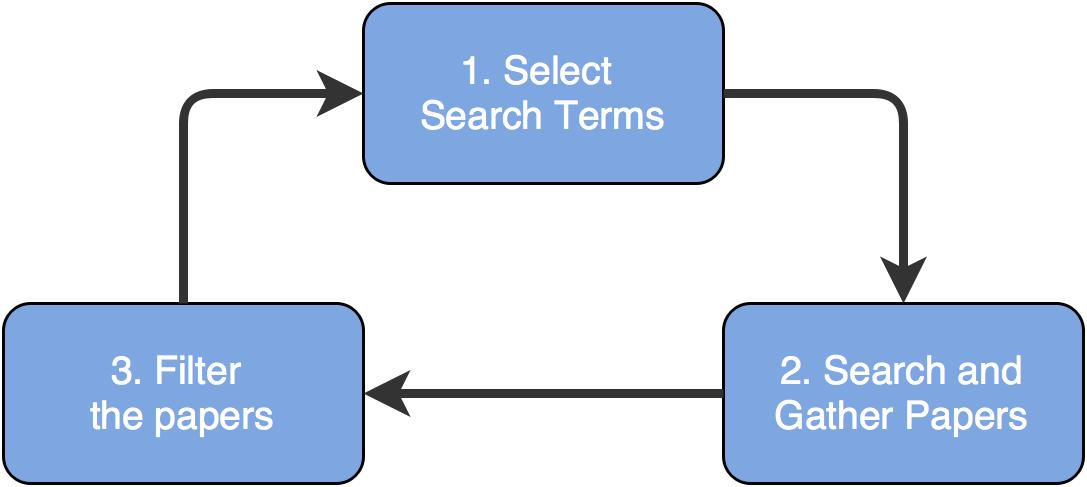
\includegraphics[width=0.8\textwidth]{figures/introduction_data_collection_phase}
\caption{Data Collection Phase}
\label{fig:context/data_collection_phase}
\end{center}
\end{figure}

\begin{enumerate}
\item \textbf{Select Search Terms}\\
At first, various search terms which define the research topics and questions are selected using the following strategies.
\begin{enumerate}
\item keywords from research questions and various definitions
\item synonyms of keywords
\item accepted and popular terms from academics and industries
\item references discovered from selected papers
\end{enumerate}
A consise list of initial keywords which are selected from various definitions of microservices are listed in Table \ref{tab:context/microservices_architecture_style/keywords_extracted_from_various_definitions_of_microservice}.
\item \textbf{Search and Gather Papers}\\
The search terms selected in the previous step are utilized to discover various research papers. In order to achieve that, the search terms are used against various resources listed below.
\begin{enumerate}
\item google scholar
\item IEEExplore
\item ACM Digital Library
\item Researchgate
\item Books
\item Technical Articles
\end{enumerate}
\item \textbf{Filter the Papers}
Finally, the research papers collected from various resources are filtered first to check if they have profound base to back up their result. Using only authentic papers is important to provide rational base to the current research. The various criteria used to filter the papers are listed below.
\begin{enumerate}
\item Is the paper relevant to answer the research question?
\item Does the paper have a good base in terms of sources and provide references of the past studies? 
\item Are there any case studies or examples provided to verify the result of the reseach?
\end{enumerate}
\end{enumerate}

\subsection{Data Synthesis Phase}\label{section:context/approach/data_synthesis_phase}
During the data synthesis phase, data is gathered from the selected research papers to create meaningful output and provide direction to the research. The Figure \ref{fig:context/data_synthesis_phase} shows various steps within this phase.

\begin{figure}[H]
\begin{center}
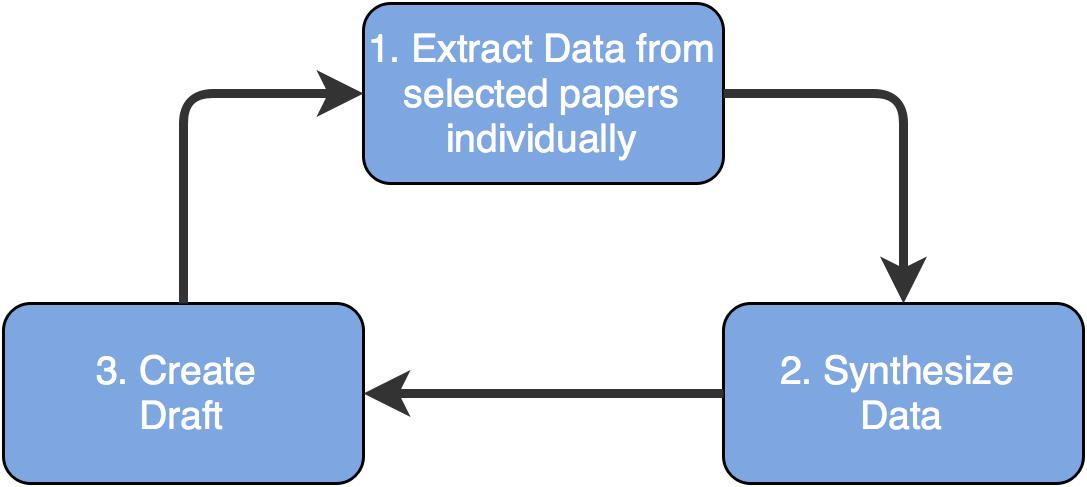
\includegraphics[width=0.8\textwidth]{figures/introduction_data_synthesis_phase}
\caption{Data Synthesis Phase}
\label{fig:context/data_synthesis_phase}
\end{center}
\end{figure}

\begin{enumerate}
\item \textbf{Extract Data from selected papers individually}\\
Firstly, each research paper is scanned and important data relevant to research are collected.
\item \textbf{Synthesize Data}\\
The data collected from each paper are revised and compared for their similarities in concepts as well as differences in opinion. These individual content from all research papers are then synthesized.
\item \textbf{Create Draft}\\
Finally, draft for the observations are created for future reference which will be used later for creating the final report.
\end{enumerate}


\section{Research Strategy}\label{section:context/research_strategy}
The Section \ref{section:context/approach} emphasizes the importance of having a consistent research procedure. It focusses on how to conduct a research in a consistent manner. In addition, it is equally important to understand what to research. A good strategy for achieving goals of the research. A good strategy is to narrow down the areas for conducting research. In this section, a list of areas is identified.\\
The various definitions in Section \ref{section:context/microservices_architecture_style/definitions} show that the authors have their own interpretation of microservices but at the same time agree upon some basic concepts. Nevertheless, each definition can be used to understand different aspect of the microservices. A distinct set of keywords can be identified from these definitions which represents different aspects. The Table \ref{tab:context/microservices_architecture_style/keywords_extracted_from_various_definitions_of_microservice} shows various keywords to focus. Additionally, there are other columns in the table which represents various aspects of microservices architecture. These columns are checked or unchecked to represent the relevance of each keyword. 

\begin{table}[H]
  \centering
  \begin{adjustbox}{max width=\textwidth}
  \begin{tabular}{*{14}{|c}|}%%{|c|c|c|c|c|c|}
  \hline
  \# & keywords & size & Quality of good microservice & communication & process to model microservices\\
  \hline
  \hline
   1 & Collaborating Services                                       &   &   & \checkmark &  \\ \hline
   2 & Communicating with lightweight mechanism like http           &   &   & \checkmark &  \\ \hline
   3 & Loosely coupled, related functions                           &   & \checkmark  & \checkmark &   \\ \hline
   4 & Developed and deployed independently       &  &   &  & \checkmark \\ \hline
   5 & Own database                                 &  & \checkmark &  & \checkmark \\ \hline
   6 & Different database technologies         &  &  &  & \checkmark \\ \hline
   7 & Service Oriented Architecture  & & \checkmark &  & \checkmark \\ \hline
   8 & Bounded Context  & \checkmark & \checkmark &  & \checkmark \\ \hline
   9 & Build around Business Capabilities  & \checkmark & \checkmark &  &\checkmark \\ \hline
   10 & Different Programming Languages & &  & & \checkmark \\ \hline
   \hline
   \end{tabular}
\end{adjustbox}
  \caption{Keywords extracted from various definitions of Microservice}
  \label{tab:context/microservices_architecture_style/keywords_extracted_from_various_definitions_of_microservice}
\end{table}
Finally, the first group of areas to focus are various aspects shown in columns such as size, quality of microservices etc.
\\
The next group of areas which need to be understood, are various drivers for defining microservices architecture. According to \cite{Brown:2015aa}, the important drivers for software architecture are: 
\label{list:introduction/drivers}
\begin{enumerate}
\item \textbf{Quality Attributes}\\
The non-functional requirements have high impact on the resulting architecture. It is important to consider various quality attributes to define the process of architecture.
\item \textbf{Constraints}\\
There are always limitations or disadvantages faced by any architectural approach.  The better knowledge of the constraint and moreover the solution to these constraints is useful in the process of explaining the architecture.
\item \textbf{Principles}\\
The various principles provides a consistent approaches to tackle various limitations. They are the keys to define guidelines.
\end{enumerate}
So, in order to define the process of modeling microservices, the key aspects related to \textbf{quality attributes}, \textbf{constraints} and \textbf{principles} is studied thoroughly.
\\
\\
Considering both the Table \ref{tab:context/microservices_architecture_style/keywords_extracted_from_various_definitions_of_microservice} and List \ref{list:introduction/drivers}, the first area to understand are various quality attributes influencing microservices architecture. Additionally, the process of identifying and modeling individual microservices from problem domain is defined. These areas are first researched based on various academic research papers. Then, the approach used by the industry for adopting microservices architecture is studied in order to answer the research questions. The industrial case study is performed in SAP Hybris.
Finally, the various constraints and challenges which affect microservices are identified. 
The results of the previous research is used to create various principles for implementing microservices architecture. These principles provide sufficient ground to create guidelines for modeling and operating microservices.

\section{Summary}\label{section:context/problem_statement}
Considering the case that the size of microservice is an important concept and is discussed a lot, but there is no concrete answer about what defines the size of a microservice. Moreover, the idea of size has a lot of interpretations and no definite answer regarding how small a microservice should be. So, the first step is to understand the concept of granularity in the context of microservices.